% This is text associated with the open textbook "Open Electromagnetics"
% See immediately below for author, date
% This work is licensed under the Creative Commons Attribution-ShareAlike 4.0 International License. (CC BY-SA 4.0) 
% To view a copy of the license, visit http://creativecommons.org/licenses/by-sa/4.0/

%ORB TITLE Single-Reactance Matching
%ORB AUTHOR 0        # S.W. Ellingson, Virginia Tech (ellingson@vt.edu)
%ORB DATE 20180802   # yyyymmdd
%ORB ABSTRACT Impedance matching using TL to match real part and then discrete impedance to match imaginary part

\label{m00093_Single-Reactance_Matching} % <-- Must match name of this file and module directory name.  Don't mess with this!
\index{impedance!matching|(}

An impedance matching structure can be designed using a section of transmission line combined with a discrete reactance, such as a capacitor or an inductor.
In the strategy presented here, the transmission line is used to transform the real part of the load impedance or admittance to the desired value, and then the reactance is used to modify the imaginary part to the desired value.
(Note the difference between this approach and the quarter-wave technique described in Section~\ref{m0091_Quarter-Wavelength_Transmission_Line}. In that approach, the first transmission line is used to zero the imaginary part.) 
There are two versions of this strategy, which we will now consider separately.

The first version is shown in Figure~\ref{m0093_fSRMs}.
The purpose of the transmission line is to transform the load impedance $Z_L$ into a new impedance $Z_1$ for which Re\{$Z_1$\} $=$ Re\{$Z_{in}$\}.
This can be done by solving the equation (from Section~\ref{m0087_Input_Impedance_of_a_Terminated_Lossless_Transmission_Line})
%
\begin{equation}
\mbox{Re}\left\{Z_1\right\} = \mbox{Re}\left\{Z_0 \frac{ 1 + \Gamma e^{-j2\beta l} }{ 1 - \Gamma e^{-j2\beta l} }\right\}
\label{m0093_eZin}
\end{equation}
%
for $l$, using a numerical search, or using the Smith chart.\footnote{For more about the Smith chart, see ``Additional Reading'' at the end of this section.}
The characteristic impedance 
\index{characteristic impedance}
$Z_0$ 
and phase propagation constant $\beta$ 
of the transmission line are independent variables and can be selected for convenience.
Normally, the smallest value of $l$ that satisfies Equation~\ref{m0093_eZin} is desired.
This value will be $\le\lambda/4$ because the real part of $Z_1$ is periodic in $l$ with period $\lambda/4$.
%
\begin{figure}
\begin{center}
\pdftooltip{{  % note double braces
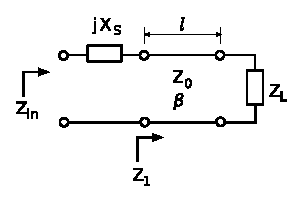
\includegraphics[width=2.5in]{modules/m0093_fSRMs.eps}
}}{A transmission line with three nodes on both the input and output branches. Starting at the top left and going clockwise, a transmission line labeled j * X sub s is between the source terminal and the middle terminal. The length between the middle terminal and the impedance terminal is measured l. Z sub 0 is measured across the terminals on either side of the impedance, with beta underneath. An arrow pointed toward the impedance originating at the middle terminal on the bottom side is labeled Z sub 1.}
\end{center} 
\caption{\label{m0093_fSRMs}Single-reactance matching with a series reactance.}
\end{figure}

After matching the real component of the impedance in this manner, the imaginary component of $Z_1$ may then be transformed to the desired value (Im\{$Z_{in}$\}) by attaching a reactance $X_s$ in series with the transmission line input, yielding $Z_{in} = Z_1 + jX_S$.  Therefore, we choose 
%
\begin{equation}
X_s = \mbox{Im}\left\{Z_{in}-Z_1\right\}
\end{equation}
%
The sign of $X_s$ determines whether this reactance is a capacitor ($X_s<0$) or inductor ($X_s>0$), and the value of this component is determined from $X_s$ and the design frequency.

%ORB EXAMPLE
~\\ \begin{example} 
\label{m0093_eSSR-S}
\begin{mdframed}[backgroundcolor=brown!20,linecolor=brown!20]\raggedright
Single reactance in series.
\\~\\
Design a match consisting of a transmission line in series with a single capacitor or inductor that matches a source impedance of $50\Omega$ to a load impedance of $33.9 + j17.6~\Omega$ at 1.5~GHz. 
The characteristic impedance and phase velocity of the transmission line are $50\Omega$ and $0.6c$ respectively.

{\bf Solution.}
From the problem statement: 
$Z_{in} \triangleq Z_S = 50~\Omega$ and 
$Z_L = 33.9+j17.6~\Omega$ are the source and load impedances respectively at $f=1.5$~GHz.
The characteristic impedance and phase velocity of the transmission line are $Z_0=50~\Omega$ and $v_p=0.6c$ respectively. 

The reflection coefficient $\Gamma$ (i.e., $Z_L$ with respect to the characteristic impedance of the transmission line) is
%
\begin{equation}
\Gamma \triangleq \frac{Z_L - Z_0}{Z_L + Z_0} \cong -0.142 + j0.239
\end{equation} 
%
The length $l$ of the primary line (that is, the one that connects the two ports of the matching structure) is determined using the equation:
%
\begin{equation}
\mbox{Re}\left\{Z_1\right\} = \mbox{Re}\left\{Z_0 \frac{ 1 + \Gamma e^{-j2\beta l} }{ 1 - \Gamma e^{-j2\beta l} }\right\}
\end{equation}
% 
where here
$\mbox{Re}\left\{Z_1\right\}=\mbox{Re}\left\{Z_S\right\}=50~\Omega$.
So a more-specific form of the equation that can be solved for $\beta l$ (as a step toward finding $l$) is:
%
\begin{equation}
1 = \mbox{Re}\left\{ 
           \frac{ 1+\Gamma e^{-j2\beta l } }
                { 1-\Gamma e^{-j2\beta l } } \right\} 
\end{equation}
%
By trial and error (or using the Smith chart if you prefer) we find $\beta l\cong 0.408$~rad for the primary line, yielding $Z_1 \cong 50.0+j29.0~\Omega$ for the input impedance after attaching the primary line.  

We may now solve for $l$ as follows:
Since $v_p = \omega/\beta$ (Section~\ref{m0080_Wave_Propagation_on_a_Transmission_Line}), we find
%
\begin{equation}
\beta = \frac{\omega}{v_p} = \frac{2\pi f}{0.6 c} \cong 52.360~\mbox{rad/m} 
\end{equation}
%
Therefore $l=\left(\beta l\right)/\beta$ $\cong$ \underline{7.8~mm}.

The impedance of the series reactance should be $jX_s \cong -j29.0~\Omega$ to cancel the imaginary part of $Z_1$.
Since the sign of this impedance is negative, it must be a capacitor.
The reactance of a capacitor is $-1/\omega C$, so it must be true that
%
\begin{equation}
-\frac{1}{2\pi f C} \cong -29.0~\Omega
\end{equation}  
%
Thus, we find the series reactance is a \underline{capacitor} of value \underline{$C\cong 3.7$~pF}.
\end{mdframed}\end{example}

\index{admittance|(}
The second version of the single-reactance strategy is shown in Figure~\ref{m0093_fSRMp}.
The difference in this scheme is that the reactance is attached in parallel.
In this case, it is easier to work the problem using admittance (i.e., reciprocal impedance) as opposed to impedance; this is because the admittance of parallel reactances is simply the sum of the associated admittances; i.e., 
%
\begin{equation}
Y_{in} = Y_1 + jB_p
\end{equation}
%
where $Y_{in}=1/Z_{in}$, $Y_1=1/Z_1$, and $B_p$ is the discrete parallel susceptance; 
\index{susceptance}
i.e., the imaginary part of the discrete parallel admittance.
%
\begin{figure}
\begin{center}
\pdftooltip{{  % note double braces
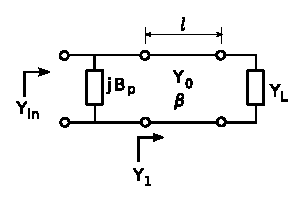
\includegraphics[width=2.5in]{modules/m0093_fSRMp.eps}
}}{A transmission line with three nodes on both the input and output branches. Starting at the top left and going clockwise, a transmission line labeled j times B sub p is connected between the source terminal and the middle terminal in parallel between input and output branches. The length between the middle terminal and the impedance terminal is measured l. Y sub 0 is measured across the terminals on either side of the impedance, with beta underneath. The impedance is labeled Y sub L. An arrow pointed toward the impedance at the middle terminal on the bottom side is labeled Y sub 1.}
\end{center} 
\caption{\label{m0093_fSRMp}Single-reactance matching with a parallel reactance.}
\end{figure}

So, the procedure is as follows.
The transmission line is used to transform $Y_L$ into a new admittance $Y_1$ for which Re\{$Y_1$\} $=$ Re\{$Y_{in}$\}.
First, we note that
%
\begin{equation}
Y_1 \triangleq \frac{1}{Z_1} = Y_0 \frac{ 1 - \Gamma e^{-j2\beta l} }{ 1 + \Gamma e^{-j2\beta l} }
\end{equation}
%
where $Y_0 \triangleq 1/Z_0$ is characteristic \emph{admittance}.
\index{characteristic admittance}
\index{admittance!characteristic|see{characteristic admittance}}
Again, the characteristic impedance $Z_0$ 
and phase propagation constant $\beta$ 
of the transmission line are independent variables and can be selected for convenience.
In the present problem, we aim to solve the equation
%
\begin{equation}
\mbox{Re}\left\{Y_1\right\} = \mbox{Re}\left\{Y_0 \frac{ 1 - \Gamma e^{-j2\beta l} }{ 1 + \Gamma e^{-j2\beta l} }\right\}
\end{equation}
%
for the smallest value of $l$, using a numerical search or using the Smith chart.
After matching the real component of the admittances in this manner, the imaginary component of the resulting admittance may then be transformed to the desired value by attaching the susceptance $B_p$ in parallel with the transmission line input. 
Since we desire $jB_p$ in parallel with $Y_1$ to be $Y_{in}$, the desired value is
%
\begin{equation}
B_p = \mbox{Im}\left\{Y_{in}-Y_1\right\}
\end{equation}
%
The sign of $B_p$ determines whether this is a capacitor ($B_p>0$) or inductor ($B_p<0$), and the value of this component is determined from $B_p$ and the design frequency.

In the following example, we address the same problem raised in Example~\ref{m0093_eSSR-S}, now using the parallel reactance approach:

%ORB EXAMPLE
~\\ \begin{example} 
\label{m0093_eSSR-P}
\begin{mdframed}[backgroundcolor=brown!20,linecolor=brown!20]\raggedright
Single reactance in parallel.
\\~\\
Design a match consisting of a transmission line in parallel with a single capacitor or inductor that matches a source impedance of $50\Omega$ to a load impedance of $33.9 + j17.6~\Omega$ at 1.5~GHz. 
The characteristic impedance and phase velocity of the transmission line are $50\Omega$ and $0.6c$ respectively.

{\bf Solution.}
From the problem statement: 
$Z_{in} \triangleq Z_S = 50~\Omega$ and 
$Z_L = 33.9+j17.6~\Omega$ are the source and load impedances respectively at $f=1.5$~GHz.
The characteristic impedance and phase velocity of the transmission line are $Z_0=50~\Omega$ and $v_p=0.6c$ respectively. 

The reflection coefficient $\Gamma$ (i.e., $Z_L$ with respect to the characteristic impedance of the transmission line) is
%
\begin{equation}
\Gamma \triangleq \frac{Z_L - Z_0}{Z_L + Z_0} \cong -0.142 + j0.239
\end{equation} 
%
The length $l$ of the primary line (that is, the one that connects the two ports of the matching structure) is the solution to:
%
\begin{equation}
\mbox{Re}\left\{Y_1\right\} = \mbox{Re}\left\{Y_{0} \frac{ 1 - \Gamma e^{-j2\beta l} }{ 1 + \Gamma e^{-j2\beta l} }\right\}
\end{equation}
% 
where here
$\mbox{Re}\left\{Y_1\right\}=\mbox{Re}\left\{1/Z_S\right\}=0.02$~mho and 
$Y_0 = 1/Z_0 = 0.02$~mho.
So the equation to be solved for $\beta l$ (as a step toward finding $l$) is:
%
\begin{equation}
1 = \mbox{Re}\left\{ 
           \frac{ 1-\Gamma e^{-j2\beta l } }
                { 1+\Gamma e^{-j2\beta l } } \right\} 
\end{equation}
%
By trial and error (or the Smith chart) we find $\beta l\cong 0.126$~rad for the primary line, yielding $Y_1 \cong 0.0200-j0.0116$~mho for the input admittance after attaching the primary line.  

We may now solve for $l$ as follows:
Since $v_p = \omega/\beta$ (Section~\ref{m0080_Wave_Propagation_on_a_Transmission_Line}), we find
%
\begin{equation}
\beta = \frac{\omega}{v_p} = \frac{2\pi f}{0.6 c} \cong 52.360~\mbox{rad/m} 
\end{equation}
%
Therefore, $l=\left(\beta l\right)/\beta$ $\cong$ \underline{2.4~mm}.

The admittance of the parallel reactance should be $jB_p \cong +j0.0116$~mho to cancel the imaginary part of $Y_1$.
The associated impedance is $1/jB_p \cong -j86.3~\Omega$.
Since the sign of this impedance is negative, it must be a capacitor.
The reactance of a capacitor is $-1/\omega C$, so it must be true that
%
\begin{equation}
-\frac{1}{2\pi f C} \cong -86.3~\Omega
\end{equation}  
%
Thus, we find the parallel reactance is a \underline{capacitor} of value \underline{$C\cong 1.2$~pF}.

\end{mdframed}\end{example}

\index{admittance|)}

Comparing this result to the result from the series reactance method (Example~\ref{m0093_eSSR-S}), we see that the necessary length of transmission line is much shorter, which is normally a compelling advantage.  The tradeoff is that the parallel capacitance is much smaller and an accurate value may be more difficult to achieve.

{\bf Additional Reading:}
\begin{itemize}
\item ``\href{https://en.wikipedia.org/wiki/Smith_chart}{\small Smith chart}'' on Wikipedia.
\end{itemize}

\index{impedance!matching|)}
